\documentclass{article}

\usepackage{amsmath}
\usepackage{amssymb}
\usepackage{parskip}
\usepackage{fullpage}
\usepackage{graphicx}
\usepackage{hyperref}
\usepackage{listings}
\usepackage{xcolor}
\usepackage{listings-rust}
\usepackage{wrapfig}

\hypersetup{
    colorlinks=true,
    linkcolor=black,
    urlcolor=blue,
    pdftitle={Paolo Bettelini - Diaries},
    pdfpagemode=FullScreen,
}

\newcommand{\wrapfill}{
    \par
    \ifnum \value{WF@wrappedlines} > 0
        \addtocounter{WF@wrappedlines}{-1}%
        \null\vspace{
            \arabic{WF@wrappedlines}
            \baselineskip
        }
        \WFclear
    \fi
}

\definecolor{background}{HTML}{EEEEEE}

\lstdefinestyle{generic} {
    backgroundcolor=\color{background},
    numbers=none,
    basicstyle=\ttfamily\color{black},
    breaklines=true,
    frame=lines
}

\title{Diaries}
\author{Paolo Bettelini}
\date{}

\begin{document}

\maketitle
\tableofcontents
\pagebreak

\section{Diaries}

\subsection{2022-12-13}

Work hours:\\
\textbf{08:20 - 11:15}: Setup and research

Today I setup the git repository with the initial files
(CLI tool, documentation, etc.).
I then spent the rest of the working
session researching the topic of the project.

The planning has yet to be done.
The goal for the next working session is to make the Gantt chart.

\subsection{2022-12-14}

Work hours:\\
\textbf{15:10 - 16:20}: Alpha matting test \\
\textbf{16:00 - 16:20}: Gantt chart

Today I started using the \texttt{opencv} library (The Rust wrapper).
I used the sample images (target and trimap) from \href{https://docs.opencv.org/4.x/dd/d0e/tutorial\_alphamat.html}{https://docs.opencv.org/4.x/dd/d0e/tutorial\_alphamat.html}.
The output is not correct, but it shows some matting to be applied.
\begin{figure}[h]
    \centering
    
\includegraphics[width=0.75\textwidth]{res1}
\end{figure}

However, I noticed a small problem: when the input images are
wrong, instead of returning \texttt{Result(Err)} (as per Rust-philosophy),
it dumps the core.

I also started making the Gantt chart.

\pagebreak

\subsection{2022-12-15}

Work hours:\\
\textbf{08:20 - 09:50}: CLI executable \\
\textbf{10:20 - 11:20}: Gantt chart

Today I fixed the trimap matting. The trimap was being read using
\texttt{IMREAD\_COLOR} rather than \texttt{IMREAD\_GRAYSCALE}.
I then added the first CLI arguments to the executabl (target image,
trimap image, output image).
I need to find a solution to avoid the core dumps from \texttt{opencv}.

\begin{figure}[h]
    \centering
    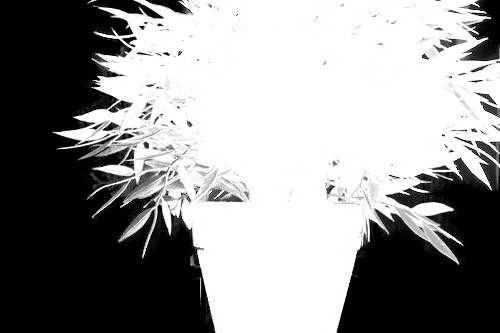
\includegraphics[width=0.75\textwidth]{res2}
\end{figure}

In the second half of the working session I completed the gantt chart

\subsection{2022-12-20}

Work hours:\\
\textbf{08:20 - 09:50}: OpenCV documentation \\
\textbf{10:20 - 11:20}: Documentation and requirements

In the first half of the working session I read
some documentation about OpenCV.
The goal is to be able to remove the background of an image
given its trimap.
In the second half I continued setting up the documentation
(requirements and layout).

\subsection{2022-12-21}

Work hours:\\
\textbf{15:05 - 15:30}: Documentation \\

Today I continued the analysis section.

\subsection{2022-12-22}

Work hours:\\
\textbf{08:20 - 09:50}: Background removal research \\
\textbf{10:05 - 10:30}: Read the review of my previous project documentation \\
\textbf{10:30 - 11:20}: GUI Research

Today I did not write any actual code, however, I did some research on which
technologies I will need to use. I realized that the background removal
cannot be done using \texttt{opencv}, but rather with another library.
Not much effort is necessary in order to finish the CLI tool, so I started
looking into the Rust GUI libraries. I also conitnued writing the requirements
in the analysis section.

The plan for the next working session is to finish the CLI tool.

\subsection{2023-01-09}

Work hours:\\
\textbf{13:15 - 16:30}: CLI

Within the last week I completed the CLI tool.
The CLI tool is capable of genering soft masks given trimaps.
It can also apply operations to images such as: making the background transparent,
filling the background with a color or replacing the background with another image.

\begin{lstlisting}[style=generic]
    Matting CLI
    
    Usage: matting-cli [OPTIONS] --target <TARGET> <--mask <MASK>|--trimap <TRIMAP>>
    
    Options:
      -i, --target <TARGET>        Target image
          --mask <MASK>            Background mask image
          --trimap <TRIMAP>        Trimap image
          --save-mask <SAVE_MASK>  Save mask path
      -o, --output <OUTPUT>        Output image
      -f, --fill <FILL>            Fill background action
      -t, --transparent            Transparent background action
      -r, --replace <REPLACE>      Replace background action
      -h, --help                   Print help information
      -V, --version                Print version information
\end{lstlisting}

The CLI tool still lacks error handling. \\
Another feature to add is the \texttt{--verbose} flag,
which prints what the program is doing along with timestamps.

\subsection{2023-01-10}

Work hours:\\
\textbf{08:20 - 9:50}: Error handling \\
\textbf{10:05 - 11:00}: Verbose flag

Today I handled every possible crash in the CLI tool.
Whenever an errors occurs it prints the according message.
I also started implemented the \texttt{--verbose} flag,
which prints program statuses and timestamps.

The plan for the next working session is to finish implementing the verbose flag.
Next, the server application can be developed.

\subsection{2023-01-11}

Work hours:\\
\textbf{15:00 - 16:20}: Verbose flag and refactor

Today I continued implementing the \texttt{--verbose} flag.
The CLI tool now prints what it is doing, but I haven't implemented the timestampts yet.
I also did some refactoring of the code and cleanup.

\subsection{2023-01-12}

Work hours:\\
\textbf{08:30 - 09:50}: CLI timestamps \\
\textbf{10:05 - 11:20}: Documentation

The CLI now fully supports the \texttt{--verbose} flag
and prints the elapsed time for each operation.

\begin{lstlisting}[style=boxed]
> matting-cli -i target.jpg --trimap trimap.png --save-mask mask.png
    --verbose -o out.png --fill red

Reading target image... Done! [4.021485ms]
Reading trimap image... Done! [1.976477ms]
Generating soft mask... Done! [7.104532642s]
Reading target image... Done! [178.884124ms]
Saving soft mask... Done! [509.050896ms]
Filling background with color... Done! [117.90393ms]
Saving output... Done! [954.085622ms]
\end{lstlisting}

I created the \lstinline[style=Rust]{log!()} macro which executes
an expression and logs a message and the elapsed time if a given flag is true.

\begin{lstlisting}[style=Rust, style=boxed]
    let mask = log!(
        "Generating soft mask",
        args.verbose,
        matting::generate_mask(&target, &trimap)? // heavy lifting
    );
\end{lstlisting}

In the second half of the working session I continued the documentation.
I did not write any actual documentation, just boilerplate and useful stuff that I'll be using.

The plan for the next working session is to crate the server worker.

\subsection{2023-01-17}

Work hours:\\
\textbf{08:30 - 11:20}: Server and API

Today I starting implementing the backend worker to process
the images. The route still does not work, althought the development
of the webserver should go smoothly after this issue.

The plan for the next working session is to continue the documentation.

\subsection{2023-01-18}

Work hours:\\
\textbf{15:00 - 16:20}: Documentation

Today I continued the documentation. I wrote the
following sections:
\begin{enumerate}
    \item \texttt{Introduction/Information}
    \item \texttt{Trimap Matting}
\end{enumerate}

\subsection{2023-01-19}

Work hours:\\
\textbf{08:30 - 10:40}: Webserver \\
\textbf{10:40 - 11:00}: Helped a classmate \\
\textbf{11:00 - 11:20}: Documentation

Today I continued working on the backend. The webserver
now serves the static webistes files. The upload root
can read the image data.

I also continued the documentation and wrote a small section
about OpenCV (\texttt{OpenCV}).

\subsection{2023-01-23}

Work hours:\\
\textbf{13:20 - 16:20}: Webserver and frontend

Today I continued working on the backend and the frontend.
The backend successfully receives POST requests containing an image
and can read its data. The frontend can load images onto the canvas
and send the canvas contents to the server. I also started
implementing the brush feature. The canvas is already capable
of simple painting features.

\subsection{2023-01-24}

Work hours:\\
\textbf{08:30 - 11:20}: Frontend Trimap Painting

Today I focused on implementing the painting feature on the frontend. \\
When an image is uploaded, I can start painting over it. There are a few settings and features such as:
\begin{itemize}
    \item Brush size slider
    \item Background / Forground selection
    \item Opacity slider
    \item Undo action
    \item Clear canvas action
\end{itemize}

I still need to implement the redo feature, and the undo features does not work if the clear feature has been
used previously. The plan for the next working session is to solely continue the documentation.

\begin{figure}[h]
    \begin{minipage}{0.5\textwidth}
        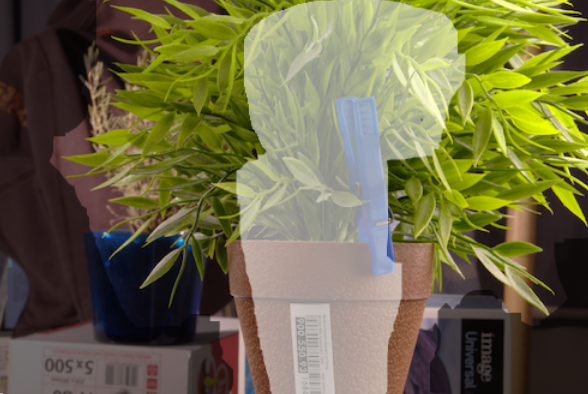
\includegraphics[width=\textwidth]{painting1.png}
    \end{minipage}
    \begin{minipage}{0.5\textwidth}
        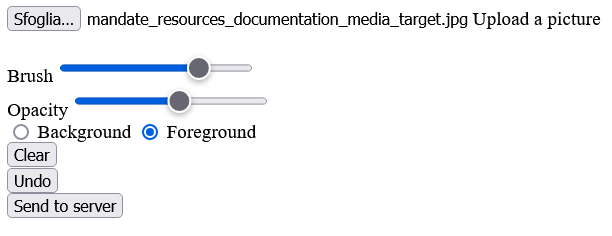
\includegraphics[width=\textwidth]{painting2.png}
    \end{minipage}
\end{figure}

\subsection{2023-01-25}

Work hours:\\
\textbf{09:05 - 10:30}: Documentation

Today I continued the documentation and wrote the following sections
\begin{itemize}
    \item \texttt{CLI/Compilation}
    \item \texttt{CLI/Usage}
    \item \texttt{CLI/Examples}
\end{itemize}

\subsection{2023-01-26}

Work hours:\\
\textbf{08:30 - 10:50}: Backend \\
\textbf{10:50 - 11:10}: Helped a classmate \\
\textbf{11:10 - 11:25}: Backend

Today I continued the backend code. The website now sends both the \texttt{target}
and \texttt{trimap} image. In the future it could just send \texttt{target} and \texttt{mask}.
The backend is able to read the data image and convert it to the \texttt{opencv} types.
Everything is ready to implement the processing logic on the backend.

\subsection{2023-01-27}

Work hours:\\
\textbf{08:30 - 09:50}: Backend \\
\textbf{12:30 - 13:50}: Backend and frontend

Today I continued the backend logic and frontend UI.
The server is still not able to generate a mask given the trimap.
In order for it to work the trimap must be processed (transparent pixels \(\rightarrow\) gray ones). \\
For now, the trimap is treated as the actual mask. The server removes the background and returns
the image to the client, which displays it on the web page.

The goal for the next session is to look into pre-processing the trimap
and continuing the web UI.

\pagebreak

\subsection{2023-01-30}

Work hours:\\
\textbf{13:15 - 13:30}: Helped a classmante \\
\textbf{13:30 - 16:20}: Frontend

Today I focused on the frontend website. I'm using the \texttt{tailwind} CSS framework
to style the page. So far the page is still a very early draft.

I plan to structure the website as follows:
\begin{enumerate}
    \item \textbf{Introductory section}: an explanation about how the process works
    \item \textbf{Upload image and trimap section}: uploading from and trimap drawing tools
    \item \textbf{Mask section}: a place to see the generated or uploaded alpha mattes mask
    \item \textbf{Transformation section}: a place to select the operation for the background
    \item \textbf{Result section}: final result display
\end{enumerate}

\subsection{2023-01-31}

Work hours:\\
\textbf{08:20 - 11:20}: Frontend

Today I continued the website code. The design is much better
and I fixed a couple of bugs:
\begin{itemize}
    \item The painting brush would draw weird spikes when moving slow
    \item The browser would keep the old input values upon a page refresh
\end{itemize}
The website now looks as follows:
\begin{figure}[ht]
    \centering
    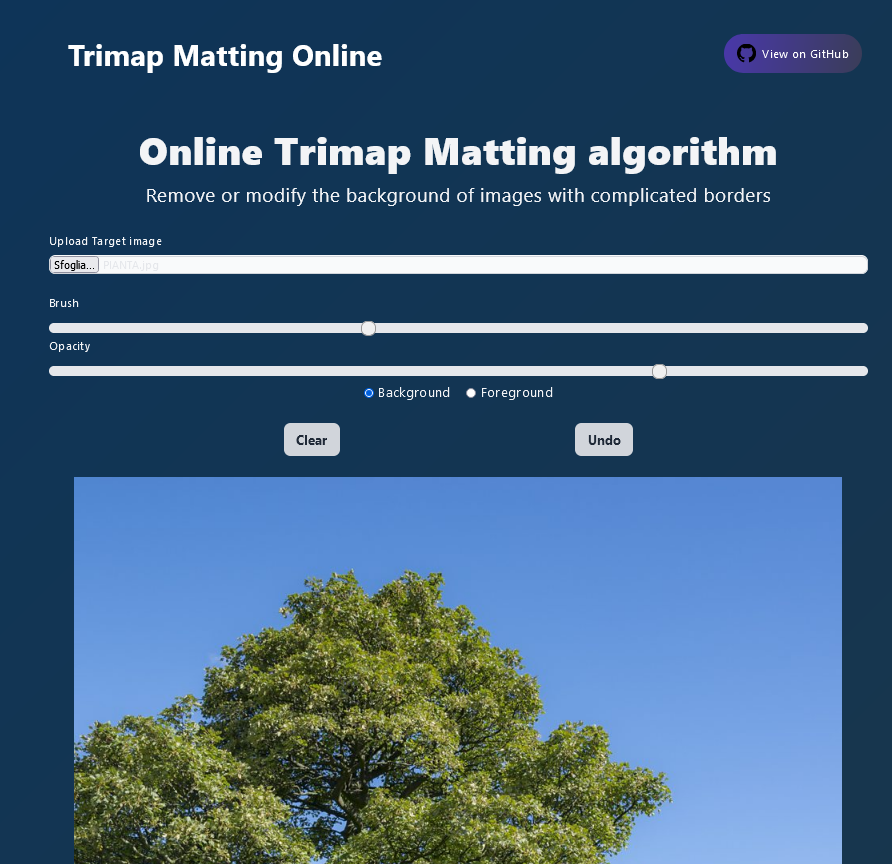
\includegraphics[width=0.60\textwidth]{web1.png}
\end{figure}

\pagebreak

\subsection{2023-02-01}

Work hours:\\
\textbf{10:50 - 12:0}: Frontend and backend

Today I started implementing the background \textit{transformation}
feature on the website. I added a form to choose between
\texttt{transparency}, \texttt{fill with color} or
\texttt{replace with image}.
I created the endpoint for this request and started implementing the logic.

The plan for the next working session is to hopefully make this feature
work.

\subsection{2023-02-02}

Work hours:\\
\textbf{08:20 - 11:40}: Frontend and backend \\
\textbf{11:40 - 12:10}: Frontend

\begin{wrapfigure}{r}{10cm}
    \vspace{-\intextsep}
    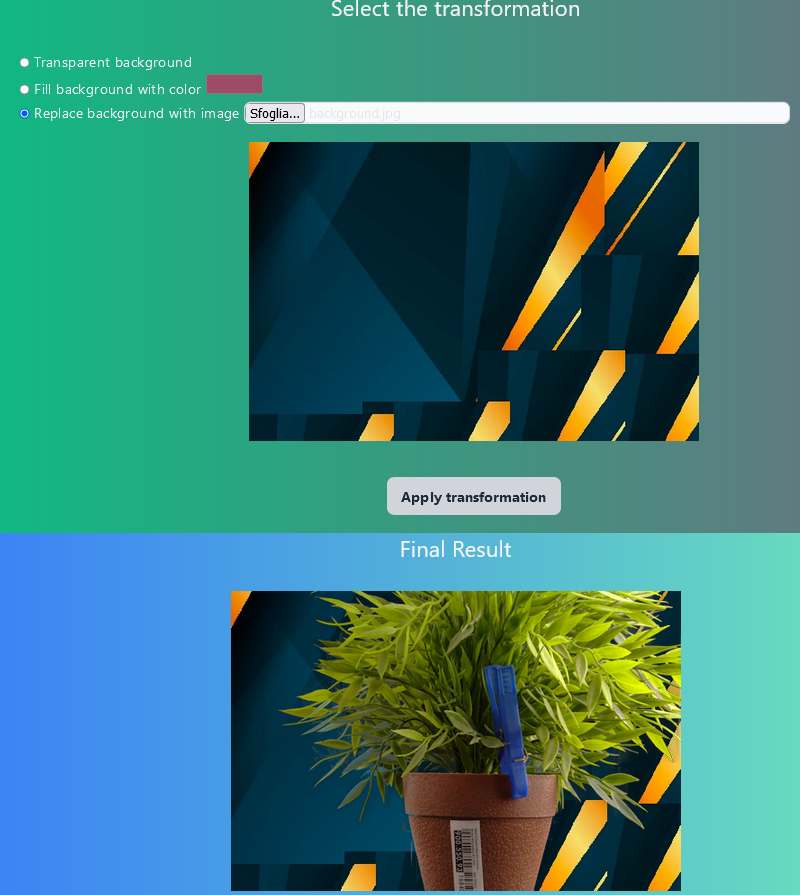
\includegraphics[width=10cm]{web2.png}
\end{wrapfigure}

Today I implemented the background operation selection on the website.
The user can choose wheter to replace the background with an image,
fill it with a color or leave it transparent.

I ended up creating 3 routes for each transformation. The routes now are
\begin{itemize}
    \item \textbf{/api/matting}
    \item \textbf{/api/fill/color}
    \item \textbf{/api/transparent}
    \item \textbf{/api/replace}
\end{itemize}

Both the backend and frontend code are a bit messy and will definitly
need some refactoring. \\
I also continued the page design a bit.

The plan for the next working session is to continue the documentation.

\wrapfill

\pagebreak

\subsection{2023-02-03}

Work hours:\\
\textbf{08:20 - 09:50}: Documentation \\
\textbf{14:20 - 15:00}: Trimap processing.

Today I continued the documentation.

\begin{itemize}
    \item Completed the \texttt{CLI/Examples} section
    \item Added missing citations
    \item Made the \texttt{Implementation} section(s)
    \item Fixed various typos
    \item Continued the \texttt{Trimap Matting} section
\end{itemize}

In the remaining time I started looking into
preprocessing the client-sent trimap.
I need to remove the alpha channel and replace the transparent pixels
with a gray color.

\subsection{2023-02-06}

Work hours:\\
\textbf{13:15 - 15:30}: Frontend \\
\textbf{15:40 - 16:30}: Research

Today I finally made the mask generation work.
I rewrote the trimap painting system a bit such that the \textit{border}
is a color (gray). However, the entire canvas is colored gray by default.

The fundamental remaining things to do are the following:
\begin{itemize}
    \item Better website design (with a loading animation)
    \item Better error handling (avoid core dumps and properly respond)
\end{itemize}

In the remaining time I did some research on how I could use the \texttt{rayon}
crate to add multithreading to my image processing functions.

\subsection{2023-02-07}

Work hours:\\
\textbf{08:20 - 11:20}: Frontend

Today I continued the frontend.
I added some logic in order to enable inputs/buttons only
when they can be used. I added the download button
under the mask image and the final result.
I also refactored some code and commented it.

\subsection{2023-02-08}

Work hours:\\
\textbf{08:20 - 11:20}: Discussed \\
\textbf{11:20 - 12:50}: Implemented changes.

Today I discussed with my supervisor about
core dumps of the opencv library and some
error handling. I started implementing some minor functionality changes
in the CLI program.

\subsection{2023-02-09}

Work hours:\\
\textbf{08:20 - 11:00}: CLI tool

Today I made some changes to the CLI tool. Namely,
if the \texttt{--output} parameter is not specified then it will
generate a name with the current timestamp (like \texttt{target\_20230209-09:52:23.jpg}). If the user
wants to save an image with transparency as something other than a \texttt{png}, he
will be warned about it.

In the second half of the working session I implemented the size checks, refactored some code,
did some tests and then read the specific requirements of the project.

\subsection{2023-02-10}

Work hours:\\
\textbf{08:20 - 09:50}: Documentation \\
\textbf{12:30 - 13:40}: Documentation

Today I continued the documentation.
I created or continued the following sections:
\begin{itemize}
    \item \texttt{Glossary}
    \item \texttt{OpenCV.Rust Binding}
    \item \texttt{OpenCV.Matting library}
\end{itemize}

I also fixed the default filename with the timestamp
(es. \texttt{target\_20230209-095223.jpg}).

\subsection{2023-02-13}

Work hours:\\
\textbf{13:15 - 16:15}: Frontend

Today I improved the frontend design (composition, titles, colors).
I fixed the autocomplete behavior of the inputs.
I also implemented the same-size check on the backend transformation
routes.

\subsection{2023-02-14}

Work hours:\\
\textbf{08:20 - 11:20}: Frontend

Today I kept developing the frontend page.
\begin{itemize}
    \item I implemented the image-size checks on the frontend.
    \item I added a loading gif when an image is processing.
    \item Better design and colors.
\end{itemize}

The plan for the next working session is to implement the bucket painting tool.
I figured it'd be very useful.

\subsection{2023-02-15}

Work hours:\\
\textbf{10:35 - 12:10}: Bucket tool

Today I started implementing the bucket/fill tool.
The algorithm works and I just need to implement it
as a feature.

\pagebreak

\subsection{2023-02-16}

Work hours:\\
\textbf{08:30 - 11:25}: Bucket tool

Today I finished implementing the fill/bucket tool.
I fixed some bugs regarding this tool, for instance,
sometimes it would go into an infinite loop.
I also added a footer to the website.

Althought the fill tool works, when an enclosed area is filled,
a thin layer of pixels of the color that's being replaced
would remain at the border of the enclosed area.
This is due to sub-pixel rendering/anti-aliasing. It would be best both for the trimap
and the flood fill not to have anti-aliasing.
I could not turn it off and instead implemented a more tolerant
algorithm which only checks if the nearest pixel is
one of the two colors (out of three) which are not being
used to fill, rather than checking if the color is not equal
to the one of the fillage.

The plan for the next working session is to
continue the documentation and try to turn off the antialiasing.

\subsection{2023-02-17}

Work hours:\\
\textbf{08:30 - 09:50}: Documentation \\
\textbf{12:30 - 13:30}: Documentation \\
\textbf{13:30 - 14:00}: Frontend

Today I continued the documentation.
I created or modified the following sections
\begin{itemize}
    \item \texttt{OpenCV.Trimap colors}
    \item \texttt{Implementation.Website.Drawing mechanics}
    \item \texttt{Implementation.Website.Flood fill}
    \item \texttt{Implementation.Website.Undo feature}
\end{itemize}

I also tried to disable the anti-aliasing but the smoothing is still there.

The plan for the next working session is to make the server
(optionally) use the CLI tool to compute matting operations.

\subsection{2023-02-27}

Work hours:\\
\textbf{13:15 - 16:20}: No matting CLI feature

Today I rewrote the matting backend so that the server calls the
\texttt{matting} CLI program (such that core dumps don't affect
the server). \\
The old code (direct FFI) is still available as a feature (no\_matting\_cli),
which is a conditional compilation condition. (E.g. \texttt{cargo build --features no\_matting\_cli}).

However, the new implementation does not work yet. The CLI program
outputs an error "No such file or directory".

\pagebreak

\subsection{2023-03-02}

Work hours:\\
\textbf{08:20 - 11:25}: No matting CLI feature

Today I finally finished implementing the \texttt{no-matting-cli} feature.
The backend server calls the CLI tool by default. I had some problems with the
file handles and automatic temp file removal.
Now the server does not crash anymore if the opencv library dumps a core.

The plan for the next working session is to do error-handling. \\
After the next working session the focus will be solely on the documentation.

\subsection{2023-03-03}

Work hours:\\
\textbf{08:30 - 09:30}: Documentation \\
\textbf{12:30 - 13:40}: Documentation

Today I decided to postpone the error handling and continue the documentation.
I created or modified the following sections
\begin{itemize}
    \item \texttt{Implementation.Core dump handling}
    \item \texttt{Implementation.Subpixel rendering and antialiasing}
    \item \texttt{Testing.Testing protocol}
    \item \texttt{Testing.Tests result}
\end{itemize}

\subsection{2023-03-13}

Work hours:\\
\textbf{13:15 - 13:30}: Matting CLI \\
\textbf{13:30 - 16:20}: Documentation

Today I finished implementing the \texttt{matting-cli} features.
Names, if the user specifies \texttt{--save-mask} without a filename
it will generate one automatically using the timestamp.
Previously, the user either specified the path or could not save the mask.
I realized in a dream that it would probably work if I put
\texttt{Option<Option<PathBuf>>} rather than \texttt{Option<PathBuf>} as a type.

I then fixed the documentation accordingly and added more examples of the usage.

In the remaining time I started writing the test protocol.

I created or modified the following sections
\begin{itemize}
    \item \texttt{Tests.Testing protocol.CLI Tests}
    \item \texttt{Tests.Testing protocol.Website Tests}
    \item \texttt{CLI.Usage}
    \item \texttt{CLI.Examples}
\end{itemize}

In the next working session I will continue
the documentation.

\pagebreak

\subsection{2023-03-14}

Work hours:\\
\textbf{08:20 - 09:50}: Matting CLI \\
\textbf{10:00 - 10:20}: Helped a classmate \\
\textbf{10:20 - 11:00}: Run tests \\
\textbf{11:00 - 11:25}: Documentation

Today I continued the documentation.
I finished the \texttt{CLI Tests} section and continued the
\texttt{Webiste Tests} one.
I also run all the tests with success.

The plan for the next working session is to finish the 
\texttt{Website Tests} section.

\subsection{2023-03-15}

Work hours:\\
\textbf{10:50 - 12:00}: Documentation \\
\textbf{12:00 - 12:15}: Helped a classmate

Today I continued the documentation. I finished writing the test
protocol for the website.

I created or modified the following sections
\begin{itemize}
    \item \texttt{Tests.Testing protocol.Website Tests}
    \item \texttt{Tests.Tests results}
\end{itemize}

The plan for the next working session is to continue the documentation.

\subsection{2023-03-16}

Work hours:\\
\textbf{08:20 - 09:20}: Fixed system \\
\textbf{09:20 - 09:50}: WebP support \\
\textbf{10:05 - 11:30}: Prepared laptop for the Swiss Skills event

Today everything broke. My system broke, the local git repository broke
and the program would not compile anymore. \\
I updated the system, fixed the repository, updated some libraries
in my code and recompiled everything a couple of times.

I then implemented support for the WebP format.
I modified the tests in the documentation accordingly.

\pagebreak

\subsection{2023-03-20}

Work hours:\\
\textbf{13:25 - 14:40}: Documentation \\
\textbf{15:00 - 16:00}: Documentation \\
\textbf{16:00 - 16:20}: CLI parameters.

Today I continued the documentation. \\
I added a requirement (default name for mask and output image).
I matched every test in the documentation to their respective
requirements and subrequirements.

I also implemented the CLI arguments for the \texttt{matting-web}
executable, which I'll document in the next working session.

I created or modified the following sections:
\begin{itemize}
    \item \texttt{Tests}
    \item \texttt{Requirements}
    \item \texttt{Conclusion.Personal conclusions}
    \item \texttt{Conclusion.Future development}
    \item \texttt{Compilation and usage.Web application.Compilation}
    \item \texttt{Compilation and usage.Web application.Usage}
\end{itemize}

\pagebreak

\subsection{2023-03-21}

Work hours:\\
\textbf{08:25 - 11:20}: Documentation

Today I continued the documentation.
I fixed some typos and rearranged some sections a bit.

I created or modified the following sections:
\begin{itemize}
    \item Structure
    \item Technologies.OpenCV
    \item Implementation.Dependencies
\end{itemize}

I also started drawing some flow charts for the documentation.

\subsection{2023-03-22}

Work hours:\\
\textbf{08:20 - 09:50}: Meeting with my advisor \\
\textbf{11:35 - 12:12}: Fixing the log system

Today I fixed the logging system in the CLI program.

The plan for the next working session is to also fix it for the Web application
and document everything logging-related.

\subsection{2023-03-23}

Work hours:\\
\textbf{08:20 - 09:50}: CLI logging documentation \\
\textbf{10:05 - 10:40}: Helped a classmate \\
\textbf{10:40 - 11:25}: WEB logging and documentation

I created or modified the following sections:
\begin{itemize}
    \item Implementation.Logging.Enviromental variables
    \item Implementation.Logging.matting-cli
    \item Implementation.Logging.matting-web
\end{itemize}

\subsection{2023-03-24}

Work hours:\\
\textbf{08:20 - 09:50}: WEB logging and error handling \\
\textbf{12:30 - 13:00}: WEB logging and error handling \\
\textbf{13:00 - 13:53}: Refactor

Today I implemented the logging system on the matting-web program.
I also handled almost every possible error with the respective logs and HTTP responses.
The program can log to a file instead of the standard output.
I also did a huge refactor: formatting, code/file separation and simplified some code.
Everything is much cleaner and more reaable.

The plan for the next working session is to continue the documentation.

\subsection{2023-03-27}

Work hours:\\
\textbf{13:15 - 16:20}: Documentation

Today I continued the documentation.
I changed the style of the test cases (include colors of the logs)
and added two test cases. I also added a requirement (logging)
and modified the usage section.

I created or modified the following sections:
\begin{itemize}
    \item Requirements
    \item Compilation and usage.CLI.Usage
    \item Compilation and usage.Web application.Usage
    \item Tests.Testing protocol
\end{itemize}

\subsection{2023-03-28}

Work hours:\\
\textbf{08:30 - 11:20}: Swim lane

Today I spent the whole time drawing swim lane diagrams. \\
There are still a couple of things I need to figure out. \\
I will hopefully start drawing them digitally in the next
working session.

\subsection{2023-03-29}

Work hours:\\
\textbf{10:50 - 11:10}: Meeting with my advisor \\
\textbf{08:30 - 11:20}: Swim lane

Today I started drawing the swim lane diagrams in a digital format. \\
I will keep doing so in the next working session.
I will also create the handled errors table in the documentation.

\subsection{2023-03-30}

Work hours:\\
\textbf{08:20 - 11:00}: Swim lane \\
\textbf{11:20 - 11:20}: Helped a classmate

Today I digitally drew the swim lane diagrams.
I had some problems with the drawing program.
The diagrams are done and I just need to format them
into the documentation with errors table.

\subsection{2023-03-31}

Work hours:\\
\textbf{08:20 - 10:30}: Swim lane and error tables \\
\textbf{10:30 - 11:20}: Helped a classmate \\
\textbf{12:30 - 13:20}: Abstract and assets \\
\textbf{13:20 - 13:44}: Helped a classmate

Today I added the swimlane diagrams to the documentation.
Each diagrams has a list of possible errors associated
with the tasks.

I created a folder for the asset images and the
document containing the abstract.

I created or modified the following sections:
\begin{itemize}
    \item \texttt{Structure.assets}
    \item \texttt{Implementation.Flux Diagrams and Error handling}
\end{itemize}

The plan for the next working session is to add
the Gantt charts.

\subsection{2023-04-04}

Work hours: \\
\textbf{08:20 - 11:20}: Documentation

Today I continued the documentation.

I fixed a lot of typos and grammatical errors.
I included the initial gantt chart and I am working
on the final gantt chart (by reconstruction).

I also wrote the section about the server logging.

\subsection{2023-04-05}

Today I almost finished writing the documentation.
I made the website design screeshots and just need to put them
into the documentation.

I created or modified the following sections:
\begin{itemize}
    \item \texttt{Technologies.Rust}
    \item \texttt{Implementation.Website.Design}
    \item \texttt{Implementation.Website.Features}
    \item \texttt{Tests.Test results}
\end{itemize}

The plan for the next working session is to add some comments to the code
and finish the documentation.

\end{document}